\section{Architekturentscheidung}\label{arch_decission}
Diagramm mit den Komponenten (unten aufgelistet) %TODO Architektur-Diagramm

\subsection{Spring Boot Anwendung}
Spring ist ein Framework für die Entwicklung von Applikationen in der Programmiersprache Java. Das Framework kann für alle Arten von Java-Anwendungen genutzt werden, da eine große Vielfalt an Abhängigkeiten für die unterschiedlichsten Funktionalitäten zur Verfügung steht.

Ursprünglich entsteht Spring als eine leichtgewichtige Alternative zu Java Enterprise Edition (\acs{JEE}), sodass die Komponenten der Software nicht mehr als Enterprise JavaBeans (\acs{EJB}s) sondern als einfache Java Objekte (\acs{POJO}s) realisiert werden können. Die Eigenschaften von \acs{EJB}s werden anhand von Techniken wie Dependency Injection und aspektorientierte Programmierung erreicht. Ein großer Nachteil hierbei ist jedoch der große Konfigurationsaufwand für die Entwickler. Initial erfolgte diese Konfiguration über mehrere \acs{XML}-Dateien. Ab Spring 2.5 wurde die \acs{XML}-basierte Konfiguration teilweise durch sogenannte Annotationen in den Java-Klassen ersetzt, was den Aufwand jedoch nicht sonderlich reduziert\cite{Walls2015}.

Das Ziel Spring Boot Projekts ist es genau diesen Nachteil zu beseitigen. Durch eine automatische Konfiguration können Entwickler schnell komplexere Spring-Anwendungen aufbauen, ohne auf die Konfiguration von allgemeinen Funktionalitäten achten zu müssen. Zudem ist auch das Einbinden von Spring-Abhängigkeiten stark vereinfacht\cite{Webb2013}.

Die Gründe für die Verwendung von Spring Boot als serverseitige Anwendung des Webshops sind einige. Zum einen ist im Team bereits etwas Erfahrung aus anderen Projekten vorhanden, die hier wiederverwendet werden kann. Zum anderen erleichtert Spring Boot durch das einfache Aufsetzen der Anwendung, der umfangreichen Dokumentation, sowie der großen Auswahl an Abhängigkeiten deutlich den Start mit der Umsetzung der eigentlichen Anforderungen. Besonders die Abhängigkeit \texttt{spring-boot-starter-web} ist für die Entwicklung von Webanwendungen nützlich, denn damit wird automatisch ein Webserver bzw. ein Java Servlet Container (Apache Tomcat) in das Projekt eingebettet.

\subsection{Angular 2 Frontend}

Angular 2 ist die neue, komplett umgebaute Version des Angular 1.x Frameworks. Diese Version liefert eine brandneue Architektur basierend auf Komponenten die in TypeScript implementiert werden. Bei TypeScript handelt es sich wiederum um ein von Microsoft entwickeltes Superset von JavaScript. TypeScript führt ein optionales Typsystem ein, sowie mehrere ECMAScript 6 Funktionalitäten, wie zum Beispiel Unterstützung von Interfaces, Klassen und Vererbung. Der Vorteil hierbei ist, dass die Erweiterungen von TypeScript von einem Compiler in normales JavaScript umgewandelt werden, sodass man TypeScript mit jedem Browser oder auch mit Node.js benutzen kann, solange der Code vorher kompiliert wird\cite{Deeleman2016}. 

%TODO Warum Angular 2

Eine Angular 2 Anwendung besteht im Grunde aus den folgenden Bausteinen\cite{Angular.io2017}:
\begin{itemize}
	\item \textit{Komponenten}
	\item \textit{Templates} 
	\item \textit{Module}
	\item \textit{Metadaten}
	\item \textit{Data Binding} 
	\item \textit{Direktiven}
	\item \textit{Services}
	\item \textit{Dependency Injection}
\end{itemize}

\subsubsection{Komponenten}
Komponenten sind Klassen die einen Teil der Oberfläche, die sogenannte \enquote{View} (zu Deutsch Darstellung), kontrollieren. Jede Klasse enthält Attributen und Methoden mit denen die Darstellung verändert werden kann.

\subsubsection{Templates}
Templates definieren wie die Darstellung einer Komponente genau aussieht. Hierfür wird eine erweiterte Form von \acs{HTML} verwendet. Templates können somit zum Beispiel auch Kinder einer Komponente durch besondere HTML-Tags anzeigen. 

\subsubsection{Module}
Module fassen mehrere Komponenten und Services zu einem Funktionalitäts-Block zusammen. Jede Angular Anwendung besitzt mindestens ein Modul, das sogenannte \enquote{Root Module}.

\subsubsection{Metadaten}
Geben Angular Information darüber, wie eine Klasse verarbeitet werden soll. Komponenten können erst von Angular als solche erkannt werden, wenn die Klasse die entsprechende Metadaten enthält. In TypeScript wird das mittels einem Decorator gemacht, eine Annotation die über die Klassendeklaration gesetzt wird.
%TODO Beispiel @Component

\subsubsection{Data Binding}
Mechanismus zur Zuordnung von bestimmten Teilen eines Templates zu Teile der dazugehörigen Komponente. \cref{fig:databinding} zeigt die vier Arten von Data Binding Syntax in Angular. Jede Form von Data Binding hat auch eine Richtung: von der Komponente zum Document Object Model (\acs{DOM}) im Template, vom DOM zur Komponente oder bidirektional.
\begin{figure}[ht!]
	\centering
	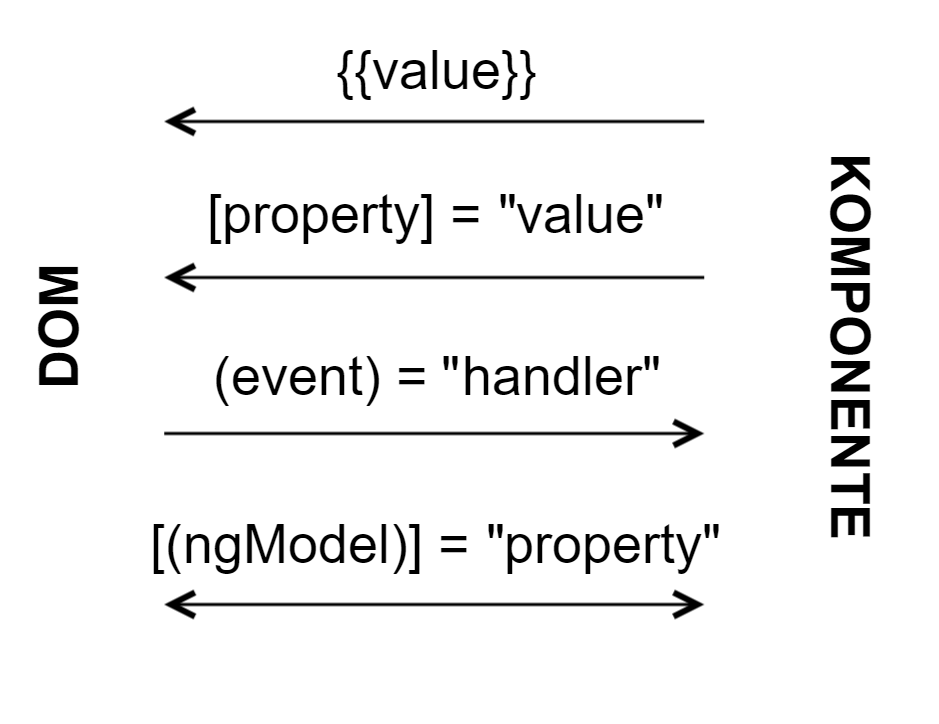
\includegraphics[width=0.4\linewidth]{bilder/kap5/databinding}
	\caption[Arten des Data Bindings in Angular 2]{Arten des Data Bindings in Angular 2\footnotemark}
	\label{fig:databinding}
\end{figure}

\footnotetext{Quelle: Angular IO, \textit{Architecture Overview - Data Binding}, 2017. URL: https://angular.io/docs/ts/latest/guide/architecture.html\#!\#data-binding}

%TODO Beispiel 

\subsubsection{Direktiven}
\subsubsection{Services}
\subsubsection{Dependency Injection}

\subsection{REST Services}
Für die Kommunikation zwischen Front- und Back-End wird REST eingesetzt. REST steht für Representational State Transfer und ist ein Architekturstil für den Entwurf von verteilten Systemen. Die Grundlage von REST wird durch folgende sechs Prinzipien festgelegt\cite{Varanasi2015}:

\begin{itemize}
	\item \textit{Client-Server}. Die Unterteilung zwischen Client und Server ermöglicht es den jeweiligen Komponenten sich unabhängig voneinander zu entwickeln und erlaubt dementsprechend die Skalierung des Systems.
	\item \textit{Zustandslos}. Die Kommunikation zwischen Client und Server sollte zustandslos sein. Das bedeutet, dass der Server sich nicht den Zustand des Clients merken braucht. Stattdessen kümmert sich der Client darum, alle notwendige Informationen in der Anfrage mitzuliefern, damit der Server diese verstehen und verarbeiten kann.
	\item \textit{Mehrschichtige Systeme}. Es können mehrere Schichten wie zum Beispiel Gateways, Firewalls oder Proxies zwischen Client und Server existieren. Diese Schichten können transparent hinzugefügt, modifiziert, umgeordnet oder gelöscht werden.
	\item \textit{Cache}. Antworten vom Server müssen als \enquote{cacheable} oder \enquote{noncacheable} deklariert sein. Dadurch wissen Clients, ob sie die Antworten zwischenspeichern können, um sie später wiederzuverwenden. Dieser Vorgang verringert die Last auf den Server und verbessert die Performance.
	\item \textit{Uniform Interface}. Alle Interaktionen zwischen Client, Server und dazwischenliegenden Komponenten basieren auf die Uniformität der Schnittstellen. Solche Schnittstellen definieren welche Ressourcen über eine eindeutige \acs{URI} durch bestimmte \acs{HTTP}-Methoden erreichbar sind. Ein Beispiel für eine REST URI könnte folgendermaßen aussehen: \\
	\texttt{http://blog.example.com/posts/1}\\
	Die URI repräsentiert hier den Zugriff auf einem Blog-Post mit Identifikator 1.
	\item \textit{Code on demand}. Clients können ihre Funktionalitäten erweitern indem sie Code (wie JavaScript Skripte oder Java Applets) bei Bedarf herunterladen und ausführen. Dies ist jedoch eine optionale Eigenschaft.
\end{itemize}

Anwendungen die diese Prinzipien befolgen, gelten als \enquote{RESTful}, also REST-konform. Es ist hierbei nicht vorgegeben, welche Technologie konkret für die Entwicklung solcher Anwendungen benutzt werden soll. Theoretisch ist es möglich eine REST-Anwendung mit einer beliebigen Netzwerk-Infrastruktur oder einem beliebigen Protokoll aufzubauen. In der Praxis nutzen diese Applikationen jedoch hauptsächlich die Eigenschaften der Web-Entwicklung und verwenden dementsprechend \acs{HTTP} als Übertragungsprotokoll.

Von den sechs oben beschriebenen Punkten ist das Prinzip des Uniform Interfaces das Hauptmerkmal von REST-Anwendungen, welches diese Art von Applikationen von anderen netzwerkbasierten Anwendungen unterscheidet. %TODO umschreiben

\subsection{MySQL Datenbank}
%TODO Warum MySQL? Vorkenntnisse in SQL, open source...